\documentclass[12pt,a4paper,openany]{report}

% ── Packages ──────────────────────────────────────────────
\usepackage[utf8]{inputenc}
\usepackage[T1]{fontenc}
\usepackage{lmodern}
\usepackage[margin=1in]{geometry}
\usepackage{setspace}
\onehalfspacing

\usepackage{graphicx}
\usepackage{booktabs}
\usepackage{longtable}
\usepackage{array}
\usepackage{tabularx}
\usepackage{multirow}
\usepackage{enumitem}
\usepackage{amsmath,amssymb}
\usepackage{float}
\usepackage{eurosym}

\usepackage[dvipsnames,table]{xcolor}
\usepackage{listings}
\usepackage[ruled,vlined,linesnumbered]{algorithm2e}

\usepackage[hidelinks]{hyperref}
\usepackage{url}
\usepackage[numbers,sort&compress]{natbib}
\usepackage{caption}
\usepackage{subcaption}
\usepackage{parskip}
\usepackage{tikz}
\usetikzlibrary{shapes.geometric, arrows.meta, positioning, fit, calc}

% ── Listings config ───────────────────────────────────────
\lstset{
  basicstyle=\ttfamily\small,
  breaklines=true,
  frame=single,
  backgroundcolor=\color{gray!8},
  keywordstyle=\color{blue!70!black}\bfseries,
  commentstyle=\color{green!50!black},
  stringstyle=\color{red!60!black},
  numbers=none,
  showstringspaces=false,
  tabsize=2,
  xleftmargin=0.5cm,
  xrightmargin=0.5cm,
}
\lstdefinelanguage{json}{
  morestring=[b]",
  morecomment=[l]{//},
}

% ══════════════════════════════════════════════════════════
\begin{document}

% ── Custom Title Page ─────────────────────────────────────
\begin{titlepage}
\centering

\vspace*{1cm}

{\LARGE\bfseries Web-Based Educational Game for\\[0.3cm]Hotel Revenue Management}\\[1.5cm]

{\large\bfseries Rajiv Gandhi Institute of Petroleum Technology}\\[0.3cm]
{\large Department of Computer Science and Engineering}\\[2.5cm]



{\large BTP - Final Report}\\[3cm]

\begin{tabular}{rl}
\textbf{Submitted by:} & Nikhilesh Raj Singh \\
\textbf{Roll No:}       & 22IT3026 \\[0.8cm]
\textbf{Supervisor:}    & Dr.\ Debashish Jena \\
\end{tabular}

\vfill

{\large April 2026}

\end{titlepage}

\newpage
\setcounter{page}{1}
\pagenumbering{roman}

% ─────────────────────────────────────────────────────────
% ABSTRACT
% ─────────────────────────────────────────────────────────
\begin{abstract}
Revenue Management (RM) is a foundational competency in the hospitality industry, yet traditional pedagogical approaches---textbooks, case studies, and static Excel models---fail to develop the real-time decision-making intuition that practitioners require. This project presents a \textbf{multiplayer web-based educational simulation game} that bridges this gap by combining machine learning models trained on 261,337 real-world hotel booking records with an interactive, real-time gaming experience.

The system comprises three main components: (1)~a~\textbf{Python ML pipeline} with five sub-models---demand~volume (Negative Binomial), guest~profiling (empirical distributions + CTGAN synthesis), ADR~prediction (LightGBM, $R^2 = 0.64$), cancellation~risk (LightGBM + Platt calibration, AUC-ROC\,=\,0.887), and no-show~prediction (AUC-ROC\,=\,0.822); (2)~a~\textbf{Node.js game backend} with Express REST~API, Socket.io real-time communication, MySQL persistent storage, and Redis ephemeral state management; and (3)~a~\textbf{React frontend} with Claymorphism UI~design, interactive KPI~dashboards, AI~benchmark comparison, and educational insights.

Evaluation confirms CTGAN-generated profiles achieve 87.84\% quality (SDV metric), Platt-scaled cancellation probabilities show mean calibration gap $<3\%$, and the end-to-end pipeline produces demand consistent with real-world patterns (5/6 criteria within $\pm$20\%). Backend verification confirms all 10 subsystems pass 50 automated checks.

\medskip\noindent
\textbf{Keywords:} Revenue Management, Gamification, Machine Learning, LightGBM, CTGAN, Probability Calibration, Educational Technology, WebSocket
\end{abstract}


% ─────────────────────────────────────────────────────────
% TABLE OF CONTENTS
% ─────────────────────────────────────────────────────────
\tableofcontents

\newpage
\setcounter{page}{1}
\pagenumbering{arabic}

% ═════════════════════════════════════════════════════════
% CHAPTER 1: INTRODUCTION
% ═════════════════════════════════════════════════════════
\chapter{Introduction}
\label{ch:intro}

Revenue Management (RM) involves strategic control of inventory, pricing, and distribution to maximize revenue per available room (RevPAR). Hotel managers make real-time decisions under uncertainty, balancing occupancy against ADR, managing cancellation risk, and optimizing room allocation across tiers.

This project shows a \textbf{multiplayer web-based educational simulation game} where players act as hotel revenue managers. ML models trained on real booking data generate realistic guest requests with pricing, risk indicators, and strategic attributes. Players decide in real time whether to accept or reject each guest, receiving feedback via leaderboards, occupancy metrics, and AI benchmark comparisons.

The system integrates \textbf{five trained sub-models} (demand volume, customer profiling, ADR prediction, cancellation risk, and no-show probability) with a CTGAN-based synthetic generator producing correlated guest profiles that mirror real-world booking patterns.

\vspace{-10pt}

\section{Key Contributions}

\begin{enumerate}
  \item \textbf{ML-Driven Simulation Engine:} A Python pipeline that transforms 261,337 historical booking records into actionable game parameters.
  \item \textbf{Dual-Path Inference Architecture:} A Python FastAPI microservice for primary CTGAN-based inference, with a Node.js ONNX fallback for resilience.
  \item \textbf{Real-Time Multiplayer Game:} Socket.io-powered game loop with concurrent player support, timed decisions, and live leaderboards.
  \item \textbf{Educational Analytics:} Post-game insights with KPI dashboards, strategy profiling, and AI benchmark comparison.
\end{enumerate}

% ═════════════════════════════════════════════════════════
% CHAPTER 2: LITERATURE REVIEW
% ═════════════════════════════════════════════════════════
\chapter{Literature Review}
\label{ch:litreview}

\section{Revenue Management in the Hospitality Industry}

RM originated in the airline industry following deregulation in the 1970s and was adapted to hotels in the late 1980s \cite{talluri2004}. The core challenge: sell the right room, to the right customer, at the right price, at the right time---under uncertain demand and perishable inventory \cite{kimes1989}. Cross (1997) showed systematic RM yields 3--7\% revenue improvement \cite{cross1997}, while Ivanov \& Zhechev (2012) confirmed hotels with formalized RM achieve significantly higher RevPAR \cite{ivanov2012}.

\section{Machine Learning in Hotel Demand Forecasting}

Modern approaches leverage ML over traditional time series methods:

\begin{itemize}
  \item \textbf{Gradient Boosting:} Ke et al.\ (2017) introduced LightGBM, now dominant for tabular prediction due to speed and accuracy \cite{ke2017}.
  \item \textbf{Cancellation Prediction:} Antonio et al.\ (2019) demonstrated gradient boosting outperforms logistic regression for hotel cancellation prediction (AUC-ROC 0.85--0.90) \cite{antonio2019}.
  \item \textbf{Probability Calibration:} Platt (1999) introduced sigmoid calibration for well-calibrated probabilities \cite{platt1999}; Niculescu-Mizil \& Caruana (2005) showed boosted trees particularly benefit from post-hoc calibration \cite{niculescu2005}.
\end{itemize}

\section{Synthetic Data Generation with GANs}

Generative Adversarial Networks \cite{goodfellow2014} have been adapted for tabular data synthesis. Xu et al.\ (2019) introduced \textbf{CTGAN} (Conditional Tabular GAN), which uses mode-specific normalization and conditional training to handle mixed-type (continuous + categorical) tabular data---a key challenge that image-focused GANs cannot address \cite{xu2019}.

The \textbf{SDV (Synthetic Data Vault)} framework \cite{patki2016} provides CTGANSynthesizer with built-in quality metrics (column shape score, column pair trends, data validity) for evaluating synthetic data fidelity.

\section{Gamification in Higher Education}

Gamification---applying game elements to non-game contexts---has shown significant positive effects on learning outcomes \cite{hamari2014}. In business education specifically:

\begin{itemize}
  \item \textbf{CAPSIM} and \textbf{Marketplace Simulations} provide multi-round business strategy games but lack industry-specific ML-driven demand models.
  \item \textbf{Hospitality-specific simulations} remain limited to Excel-based exercises with predetermined scenarios \cite{kim2015}.
  \item \textbf{Serious games} have been proposed for hotel management training \cite{ampatzoglou2010}, but none integrate real-world data or ML-generated demand.
\end{itemize}

\section{Real-Time Web Technologies}

WebSocket-based communication (via Socket.io) enables server-push architectures essential for multiplayer games \cite{fette2011}. Unlike HTTP polling, WebSockets maintain persistent connections, reducing latency from seconds to milliseconds---critical for timed game mechanics.

\section{Summary of Literature Gap}

\begin{table}[H]
\centering
\caption{Comparison of existing solutions with this project.}
\label{tab:litgap}
\small
\begin{tabular}{@{}lcccc@{}}
\toprule
\textbf{Feature} & \textbf{CAPSIM} & \textbf{Excel RM} & \textbf{Commercial} & \textbf{This Project} \\
\midrule
Real hotel booking data       & \texttimes & \texttimes & \texttimes & \checkmark\ 261K records \\
ML-generated demand           & \texttimes & \texttimes & \checkmark & \checkmark\ 5 sub-models \\
CTGAN synthesis               & \texttimes & \texttimes & \texttimes & \checkmark\ 87.84\% quality \\
Calibrated risk probabilities & \texttimes & \texttimes & Partial    & \checkmark\ Platt-scaled \\
Real-time multiplayer         & \texttimes & \texttimes & \texttimes & \checkmark\ Socket.io \\
Post-game AI benchmark        & \texttimes & \texttimes & \texttimes & \checkmark\ Greedy EV \\
Educational analytics         & \texttimes & \texttimes & \texttimes & \checkmark\ KPI + insights \\
Open-source / free            & \texttimes & \checkmark & \texttimes & \checkmark \\
\bottomrule
\end{tabular}
\end{table}

No existing system combines ML-trained demand models, CTGAN-based synthetic guest generation, real-time multiplayer competition, calibrated probabilistic risk assessment, and detailed post-game analytics. This project fills this gap.


% ═════════════════════════════════════════════════════════
% CHAPTER 3: PROBLEM STATEMENT & OBJECTIVES
% ═════════════════════════════════════════════════════════
\chapter{Problem Statement \& Objectives}
\label{ch:problem}

\section{Problem Statement}

\begin{quote}
\itshape
Design and implement a multiplayer web-based educational simulation game for hotel revenue management that generates realistic guest booking scenarios using machine learning models trained on real-world hotel data, enabling players to practice real-time accept/reject decision-making while receiving quantitative performance feedback.
\end{quote}

\section{Objectives}

\begin{table}[H]
\centering
\caption{Project objectives and completion status.}
\label{tab:objectives}
\begin{tabular}{@{}clc@{}}
\toprule
\textbf{\#} & \textbf{Objective} & \textbf{Status} \\
\midrule
O1 & Build a data pipeline to clean and engineer features from 261K+ records & \checkmark \\
O2 & Train ML models for demand volume, guest profiling, ADR, cancel, no-show & \checkmark \\
O3 & Implement a CTGAN-based synthetic guest generator preserving correlations & \checkmark \\
O4 & Develop a real-time multiplayer game backend with WebSocket communication & \checkmark \\
O5 & Create an interactive frontend with Claymorphism UI for immersive gameplay & \checkmark \\
O6 & Provide post-game analytics with KPI dashboards, insights, and AI benchmarking & \checkmark \\
O7 & Formally evaluate all models with train/test metrics and calibration analysis & \checkmark \\
\bottomrule
\end{tabular}
\end{table}



% ═════════════════════════════════════════════════════════
% CHAPTER 5: PROPOSED SOLUTION & METHODOLOGY
% ═════════════════════════════════════════════════════════
\chapter{Proposed Solution \& Methodology}
\label{ch:methodology}

\section{System Architecture Overview}

The system follows a \textbf{three-tier microservice architecture} with clear separation between ML training, inference, and game logic. Figure~\ref{fig:sysarch} illustrates the high-level architecture.

\begin{figure}[H]
\centering
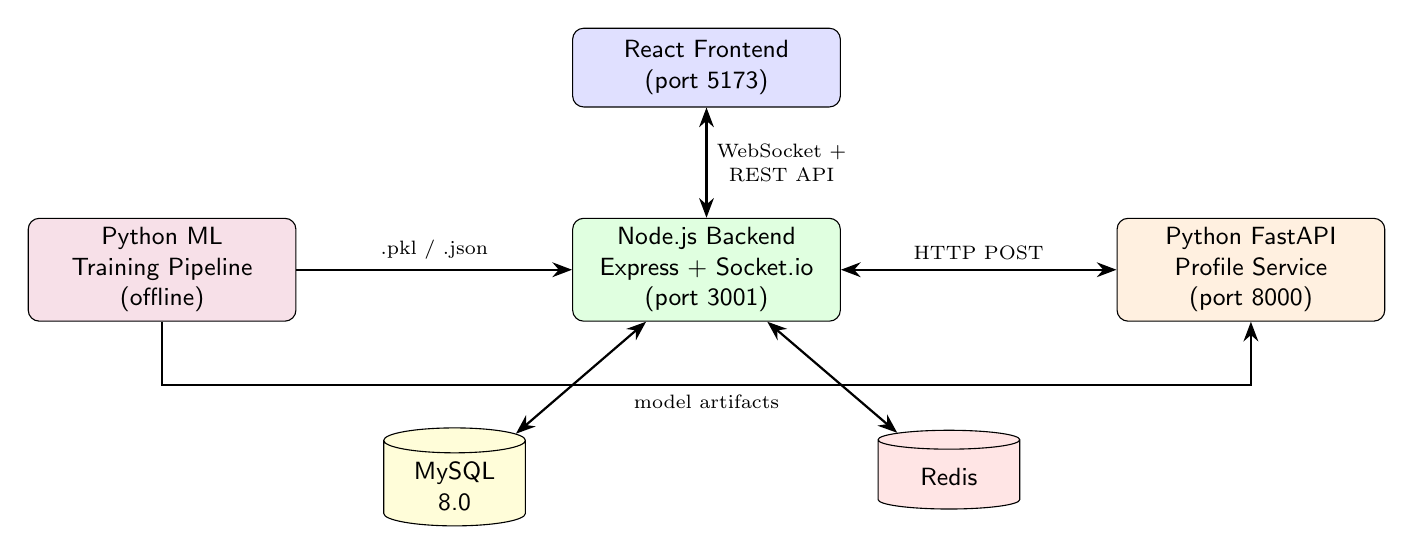
\begin{tikzpicture}[
  box/.style={rectangle, draw, rounded corners=4pt, minimum width=3.4cm, minimum height=1cm, align=center, font=\small\sffamily},
  db/.style={cylinder, draw, shape border rotate=90, minimum width=1.8cm, minimum height=1cm, align=center, font=\small\sffamily, aspect=0.25},
  arr/.style={-{Stealth[length=2.5mm]}, thick},
  darr/.style={{Stealth[length=2.5mm]}-{Stealth[length=2.5mm]}, thick},
]

% === Top row: Frontend ===
\node[box, fill=blue!12] (fe) {React Frontend\\(port 5173)};

% === Middle row: Training — Backend — Python Service ===
\node[box, fill=green!12, below=1.4cm of fe] (be) {Node.js Backend\\Express + Socket.io\\(port 3001)};
\node[box, fill=purple!12, left=3.5cm of be] (train) {Python ML\\Training Pipeline\\(offline)};
\node[box, fill=orange!12, right=3.5cm of be] (py) {Python FastAPI\\Profile Service\\(port 8000)};

% === Bottom row: Data stores ===
\node[db, fill=yellow!15, below left=1.4cm and 0.8cm of be] (mysql) {MySQL\\8.0};
\node[db, fill=red!10, below right=1.4cm and 0.8cm of be] (redis) {Redis};

% === Arrows ===
% Frontend <-> Backend (vertical)
\draw[darr] (fe) -- node[right, font=\scriptsize]{\shortstack{WebSocket +\\REST API}} (be);

% Backend <-> Python service (horizontal, clear path)
\draw[darr] (be) -- node[above, font=\scriptsize]{HTTP POST} (py);

% Backend <-> Data stores (diagonal down)
\draw[darr] (be) -- (mysql);
\draw[darr] (be) -- (redis);

% Training -> Backend (horizontal, clear path)
\draw[arr] (train) -- node[above, font=\scriptsize]{.pkl / .json} (be);

% Training -> Python service (routed BELOW to avoid crossing backend)
\draw[arr] (train.south) -- ++(0,-0.8) -| node[near start, below, font=\scriptsize]{model artifacts} (py.south);
\end{tikzpicture}
\caption{High-level system architecture.}
\label{fig:sysarch}
\end{figure}

The architecture consists of:
\begin{enumerate}
  \item \textbf{Python Training Pipeline (Offline):} Processes raw hotel data through 11 scripts, producing serialized model artifacts (JSON configs and \texttt{.pkl} models).
  \item \textbf{Python FastAPI Service (Runtime, port 8000):} Loads trained models (CTGAN, LightGBM) and exposes a \texttt{/generate-guests} API endpoint for on-demand guest profile generation.
  \item \textbf{Node.js Game Backend (Runtime, port 3001):} Express REST API + Socket.io WebSocket server; orchestrates game sessions, manages real-time decision flow, and stores results in MySQL/Redis.
  \item \textbf{React Frontend (port 5173):} Claymorphism-styled SPA with pages for authentication, dashboard, gameplay, results, KPIs, insights, and leaderboards.
  \item \textbf{Data Stores:} MySQL 8.0 for persistent data (users, sessions, bookings) and Redis for ephemeral game state (room inventories, timers).
\end{enumerate}


\section{Data Collection \& Preprocessing}

\subsection{Dataset Description}

Two complementary datasets were combined to form a 6-year historical record:

\begin{table}[H]
\centering
\caption{Source datasets.}
\label{tab:datasets}
\begin{tabular}{@{}llrl@{}}
\toprule
\textbf{Dataset} & \textbf{Period} & \textbf{Rows} & \textbf{Source} \\
\midrule
\texttt{hotel\_revenue\_historical\_full.xlsx} & 2018--2020 & 141,947 & 3 yearly sheets + 2 lookups \\
\texttt{hotel\_booking.csv}                    & 2015--2017 & 119,390 & Kaggle (4 PII columns dropped) \\
\textbf{Combined}                              & \textbf{2015--2020} & \textbf{261,337} & Merged on 32 common columns \\
\bottomrule
\end{tabular}
\end{table}

Each record represents one hotel booking with 32 features including: hotel type, lead time, arrival date, length of stay, number of guests, meal plan, market segment, deposit type, room type, ADR, cancellation status, and reservation outcome.

\subsection{Data Cleaning Pipeline}

Nine cleaning steps were applied sequentially:

\begin{table}[H]
\centering
\caption{Data cleaning steps.}
\label{tab:cleaning}
\small
\begin{tabular}{@{}clr@{}}
\toprule
\textbf{Step} & \textbf{Action} & \textbf{Rows Affected} \\
\midrule
1 & Drop room type P (ADR=0, complimentary)     & 25 removed \\
2 & Drop zero-night stays                       & 1,563 removed \\
3 & Drop negative ADR                           & 2 removed \\
4 & Cap ADR outliers at 99.5th percentile        & 1,404 clipped \\
5 & Cap LoS outliers at 99th percentile          & 1,980 clipped \\
6 & Exclude post-COVID period (Mar 2020+)        & 32,742 removed \\
7 & Drop ``Undefined'' market segment            & 6 removed \\
8 & Merge lookup tables (meal cost, discount)    & 0 \\
9 & Column selection (retain 33 columns)         & 0 \\
\bottomrule
\end{tabular}
\end{table}

\textbf{Output:} \texttt{df\_clean.csv} --- \textbf{226,999 rows $\times$ 33 columns}

\subsection{Feature Engineering}

Seventeen new features were engineered across three categories:

\textbf{Temporal Features (6):} \texttt{month\_num} (1--12), \texttt{is\_summer} (Jun--Aug), \texttt{is\_winter} (Nov--Feb), \texttt{is\_weekend\_arrival}, \texttt{total\_guests} (capped at 10), \texttt{lead\_time\_bucket} (6 ordinal buckets).

\textbf{Hotel/Room Features (5):} \texttt{hotel\_encoded} (City=0, Resort=1), \texttt{room\_tier} (4-level mapping: Standard/Mid/Premium/Suite), \texttt{assigned\_room\_tier}, \texttt{room\_was\_upgraded}, \texttt{upgrade\_delta\_tier}.

\textbf{Commercial/Behavioral Features (6):} \texttt{net\_adr}, \texttt{total\_revenue}, \texttt{has\_special\_requests}, \texttt{has\_prev\_cancellations}, \texttt{loyalty\_score} (capped at 20), \texttt{is\_non\_refund}.

\textbf{Target Variables (2):} \texttt{target\_cancel} (binary), \texttt{target\_noshow} (binary: reservation\_status == `No-Show').

\textbf{Output:} \texttt{df\_featured.csv} --- \textbf{226,999 rows $\times$ 53 columns}

\subsection{Train/Test Split}

A \textbf{temporal split} was used (not random) to simulate real-world deployment:

\begin{table}[H]
\centering
\caption{Temporal train/test split.}
\label{tab:split}
\begin{tabular}{@{}llrl@{}}
\toprule
\textbf{Set} & \textbf{Criteria} & \textbf{Size} & \textbf{Purpose} \\
\midrule
Train & \texttt{arrival\_date < 2020-01-01} (2015--2019) & 219,199 rows & Model training \\
Test  & \texttt{arrival\_date $\geq$ 2020-01-01} (Jan--Feb 2020) & 7,800 rows & Holdout evaluation \\
\bottomrule
\end{tabular}
\end{table}

\section{ML Pipeline --- Demand Generation Models}

Five sub-models form the demand generation engine:

\subsection{Sub-Model 1: Daily Demand Volume}

\textbf{Method:} Empirical Negative Binomial (method-of-moments). For each of 24 hotel $\times$ month combinations, mean ($\mu$) and dispersion ($\alpha$) are computed from daily booking counts with year-based exponential weighting (recent years weighted 4$\times$). City Hotel $\mu$ ranges from 64.4 (Jan) to 174.7 (Sep); Resort Hotel from 37.5 (Jan) to 79.6 (Oct).

\textbf{Game Balance Scaling:} Raw $\mu$ values are linearly mapped to $[5, 20]$ guests per in-game day:
\begin{equation}
\text{scaled\_mu} = 5 + \left\lfloor \frac{\mu - \mu_{\min}}{\mu_{\max} - \mu_{\min}} \times 15 \right\rceil
\end{equation}
This preserves seasonal variation while keeping gameplay manageable (30-second timer per guest).

\subsection{Sub-Model 2: Customer Profile Generator}

\textbf{Method:} Distribution fitting (no ML required). Seven profile components fitted from empirical distributions: Room Type (Multinomial), LoS (Negative Binomial), Meal Plan (Categorical), Market Segment (Categorical), Total Guests (Empirical PMF), Guest Attributes (Bernoulli), and Lead Time (Exponential Mixture).

Key differences by hotel type: City Hotel has 83.3\% Standard room share (vs.\ 61.5\% Resort), mean LoS 2.9 nights (vs.\ 4.3), non-refund rate 18.7\% (vs.\ 5.8\%), and Online TA share $\sim$40\% for both.

\subsection{Sub-Model 3: ADR (Average Daily Rate) Prediction}

\textbf{Model:} LightGBM Regressor (separate models per hotel type)\\
\textbf{Training data:} Check-Out bookings only (138,041 rows)---avoids phantom cancelled bookings\\
\textbf{Features:} 13 (\texttt{room\_tier}, \texttt{month\_num}, \texttt{los}, \texttt{market\_segment}, etc.)

Per-hotel hyperparameters: Resort Hotel gets more capacity (800 estimators, 127 leaves) vs City Hotel (500 estimators, 63 leaves) to handle higher ADR variance.

\textbf{Noise injection:} At inference, Gaussian noise ($\sigma \approx$ \texteuro{}20) ensures no two identical-profile guests have the same ADR.

\subsection{Sub-Model 4: Cancellation Risk (Binary Classification)}

\textbf{Model:} LightGBM Classifier + Platt Scaling Calibration\\
\textbf{Features:} 15 (\texttt{is\_non\_refund}, \texttt{lead\_time}, \texttt{loyalty\_score}, etc.)\\
\textbf{Calibration:} \texttt{CalibratedClassifierCV(method='sigmoid', cv=5)} ensures predicted probabilities are well-calibrated---a 70\% risk truly means $\sim$70\% of such bookings cancel.

\textbf{Risk Badge System} displayed on guest cards:
\begin{itemize}
  \item \textcolor{green!60!black}{\textbf{Green:}} $p_{\text{cancel}} < 0.25$ (low risk)
  \item \textcolor{yellow!80!black}{\textbf{Yellow:}} $0.25 \leq p_{\text{cancel}} < 0.55$ (medium risk)
  \item \textcolor{red!70!black}{\textbf{Red:}} $p_{\text{cancel}} \geq 0.55$ (high risk)
\end{itemize}

\subsection{Sub-Model 5: No-Show Prediction}

\textbf{Model:} LightGBM Classifier with \texttt{scale\_pos\_weight} $\approx 89.7$\\
\textbf{Features:} 6 (\texttt{hotel}, \texttt{lead\_time\_bucket}, \texttt{is\_non\_refund}, \texttt{market\_segment}, \texttt{month}, \texttt{total\_guests})\\
\textbf{Challenge:} Extreme class imbalance (only 1.04\% positive rate)


\section{Guest Profile Synthesis (CTGAN)}

\subsection{Why CTGAN over Independent Sampling?}

Independent statistical sampling (Sub-Model 2) treats each guest attribute independently. In reality, attributes are correlated---business travelers (Corporate segment) tend to have shorter stays, standard rooms, and lower special request rates. \textbf{CTGAN preserves these cross-feature correlations.}

\subsection{Architecture}

The CTGAN pipeline consists of a CTGANSynthesizer (generator: 256$\times$256, discriminator: 256$\times$256) trained for 150 epochs with batch size 500 and PAC=10 on Google Colab T4 GPU. Training uses 13 profile features from 219,199 rows. Conditional vectors (hotel type + month) enable conditioned sampling, producing seasonally-appropriate guest mixes at runtime.

\subsection{Guest Generation Pipeline Flowchart}

Figure~\ref{fig:ctganflow} illustrates the dual-path guest generation pipeline, from game request to complete guest object.

\begin{figure}[H]
\centering
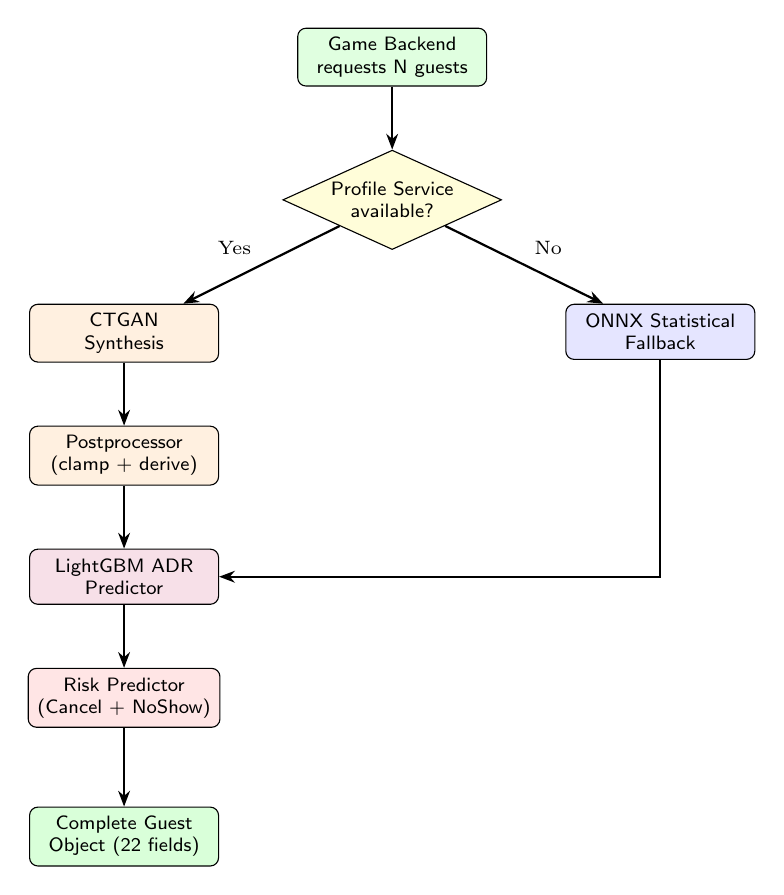
\begin{tikzpicture}[
  box/.style={rectangle, draw, rounded corners=3pt, minimum width=2.4cm, minimum height=0.7cm, align=center, font=\scriptsize\sffamily},
  decision/.style={diamond, draw, aspect=2.2, minimum width=1cm, align=center, font=\scriptsize\sffamily, inner sep=1pt},
  arr/.style={-{Stealth[length=2mm]}, thick},
]
% Start
\node[box, fill=green!12] (start) {Game Backend\\requests N guests};
\node[decision, fill=yellow!15, below=0.8cm of start] (check) {Profile Service\\available?};
\node[box, fill=orange!12, below left=1cm and 1.5cm of check] (ctgan) {CTGAN\\Synthesis};
\node[box, fill=blue!10, below right=1cm and 1.5cm of check] (onnx) {ONNX Statistical\\Fallback};
\node[box, fill=orange!12, below=0.8cm of ctgan] (post) {Postprocessor\\(clamp + derive)};
\node[box, fill=purple!12, below=0.8cm of post] (adr) {LightGBM ADR\\Predictor};
\node[box, fill=red!10, below=0.8cm of adr] (risk) {Risk Predictor\\(Cancel + NoShow)};
\node[box, fill=green!15, below=1cm of risk] (out) {Complete Guest\\Object (22 fields)};

% Arrows
\draw[arr] (start) -- (check);
\draw[arr] (check) -- node[above left, font=\scriptsize]{Yes} (ctgan);
\draw[arr] (check) -- node[above right, font=\scriptsize]{No} (onnx);
\draw[arr] (ctgan) -- (post);
\draw[arr] (onnx) |- (adr);
\draw[arr] (post) -- (adr);
\draw[arr] (adr) -- (risk);
\draw[arr] (risk) -- (out);
\end{tikzpicture}
\caption{Dual-path guest generation pipeline.}
\label{fig:ctganflow}
\end{figure}

\section{Game Backend Architecture (Node.js)}

\subsection{Layered Architecture}

The backend follows a strict \textbf{Single Responsibility Principle (SRP)} with 9 layers:

\begin{enumerate}
  \item \textbf{Routes Layer:} \texttt{auth.js}, \texttt{sessions.js} --- REST API endpoints
  \item \textbf{Socket Handlers:} \texttt{gameHandler}, \texttt{decisionHandler}
  \item \textbf{Middleware:} JWT authentication
  \item \textbf{Services Layer:} 9 services (\texttt{authService}, \texttt{sessionService}, \texttt{gameService}, \texttt{decisionService}, \texttt{pricingService}, \texttt{roomInventoryService}, \texttt{weekResolutionService}, \texttt{benchmarkService}, \texttt{leaderboardService})
  \item \textbf{Repositories Layer:} 6 repositories mapping to MySQL tables
  \item \textbf{Game Orchestrators:} \texttt{weekOrchestrator}, \texttt{guestTimerManager}
  \item \textbf{Demand Layer:} \texttt{modelLoader}, \texttt{guestFactory}, \texttt{adrPredictor}, \texttt{riskPredictor}, \texttt{profileSampler}
  \item \textbf{MySQL 8.0:} 6 tables for persistent storage
  \item \textbf{Redis:} Ephemeral state with 2-hour TTL
\end{enumerate}

\subsection{Redis Key Design}

All game state is cached in Redis with 2-hour TTL using the naming convention \texttt{session:\{id\}:*} (e.g., \texttt{:state}, \texttt{:player:\{uid\}:rooms}, \texttt{:week:\{n\}:guestTimer}). Room inventory calendars store a 7-day $\times$ 4-tier availability matrix per player. \texttt{WATCH/MULTI} transactions ensure atomic inventory updates when multiple players accept the same room tier simultaneously.

\section{Real-Time Game Loop Algorithm}

The game loop follows the sequence shown in Figure~\ref{fig:gameloop}.

\begin{figure}[H]
\centering
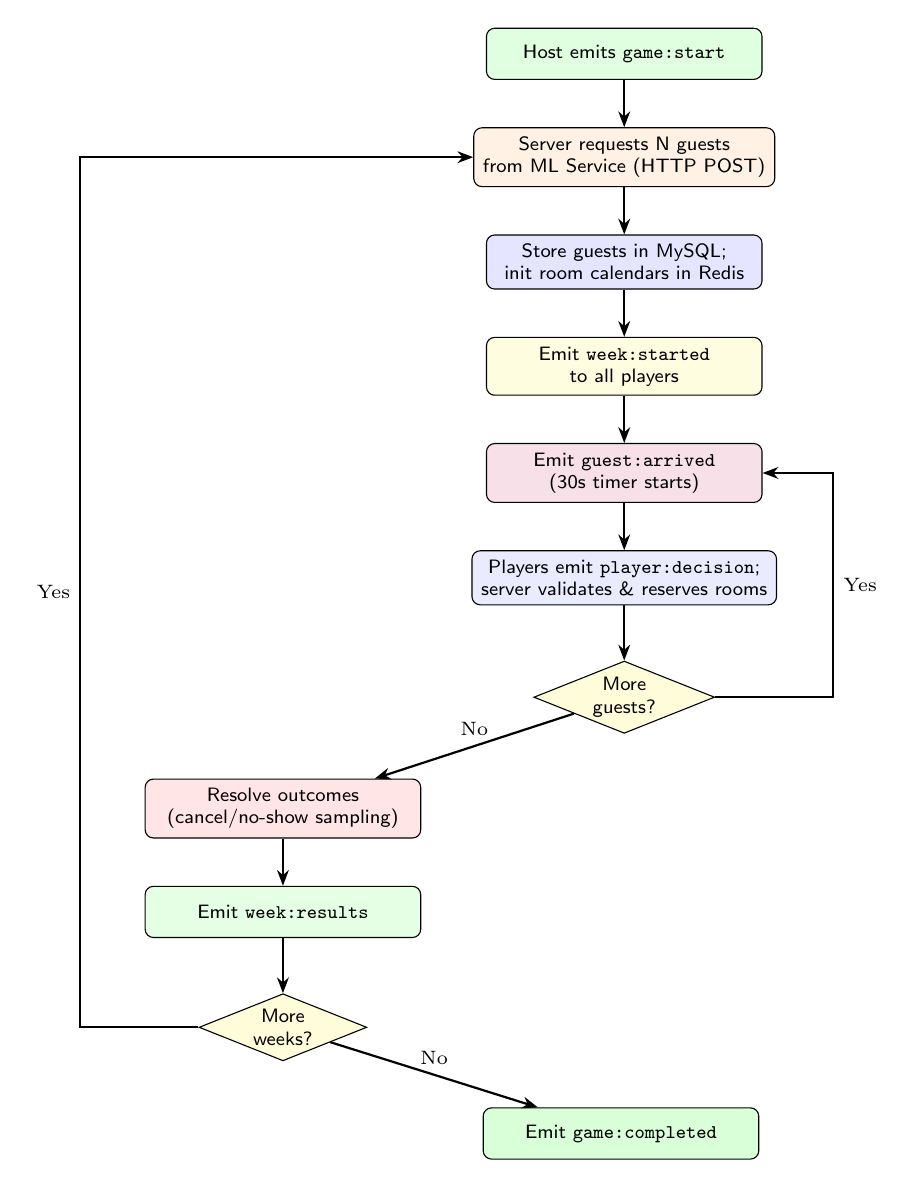
\begin{tikzpicture}[
  box/.style={rectangle, draw, rounded corners=3pt, minimum width=3.5cm, minimum height=0.65cm, align=center, font=\scriptsize\sffamily},
  decision/.style={diamond, draw, aspect=2.5, minimum width=1cm, align=center, font=\scriptsize\sffamily, inner sep=1pt},
  arr/.style={-{Stealth[length=2mm]}, thick},
]
\node[box, fill=green!12] (s1) {Host emits \texttt{game:start}};
\node[box, fill=orange!10, below=0.6cm of s1] (s2) {Server requests N guests\\from ML Service (HTTP POST)};
\node[box, fill=blue!10, below=0.6cm of s2] (s3) {Store guests in MySQL;\\init room calendars in Redis};
\node[box, fill=yellow!12, below=0.6cm of s3] (s4) {Emit \texttt{week:started}\\to all players};
\node[box, fill=purple!12, below=0.6cm of s4] (s5) {Emit \texttt{guest:arrived}\\(30s timer starts)};
\node[box, fill=blue!8, below=0.6cm of s5] (s6) {Players emit \texttt{player:decision};\\server validates \& reserves rooms};
\node[decision, fill=yellow!15, below=0.7cm of s6] (d1) {More\\guests?};
\node[box, fill=red!10, below left=0.8cm and 2cm of d1] (s7) {Resolve outcomes\\(cancel/no-show sampling)};
\node[box, fill=green!10, below=0.6cm of s7] (s8) {Emit \texttt{week:results}};
\node[decision, fill=yellow!15, below=0.7cm of s8] (d2) {More\\weeks?};
\node[box, fill=green!15, below right=0.8cm and 2cm of d2] (end) {Emit \texttt{game:completed}};

% Arrows
\draw[arr] (s1) -- (s2);
\draw[arr] (s2) -- (s3);
\draw[arr] (s3) -- (s4);
\draw[arr] (s4) -- (s5);
\draw[arr] (s5) -- (s6);
\draw[arr] (s6) -- (d1);
\draw[arr] (d1) -- node[above, font=\scriptsize]{No} (s7);
\draw[arr] (d1.east) -- ++(1.5,0) |- node[near start, right, font=\scriptsize]{Yes} (s5.east);
\draw[arr] (s7) -- (s8);
\draw[arr] (s8) -- (d2);
\draw[arr] (d2.west) -- ++(-1.5,0) |- node[near start, left, font=\scriptsize]{Yes} (s2.west);
\draw[arr] (d2) -- node[above, font=\scriptsize]{No} (end);
\end{tikzpicture}
\caption{Real-time game loop flowchart.}
\label{fig:gameloop}
\end{figure}

\subsection{Decision Processing Algorithm}

\begin{algorithm}[H]
\SetAlgoLined
\KwIn{sessionId, userId, guestIndex, decision, roomTier}
\KwOut{Updated room inventory and booking record}
Validate guest is current (not expired by timer)\;
Validate player hasn't already decided for this guest\;
\If{decision == ``accepted''}{
  guest $\leftarrow$ getCurrentGuest(sessionId, guestIndex)\;
  arrivalDay $\leftarrow$ guest.arrival\_day\;
  tierKey $\leftarrow$ TIER\_MAP[roomTier]\;
  calendar $\leftarrow$ Redis.GET(inventory key)\;
  \For{day $=$ arrivalDay \KwTo arrivalDay + guest.los $- 1$}{
    \If{calendar[day \% 7][tierKey] $\leq 0$}{
      \Return error(``No availability for this room tier'')\;
    }
  }
  Redis.WATCH(inventoryKey) \tcp*{Optimistic locking}
  \For{day $=$ arrivalDay \KwTo arrivalDay + guest.los $- 1$}{
    calendar[day \% 7][tierKey] $-= 1$\;
  }
  Redis.MULTI $\rightarrow$ SET calendar $\rightarrow$ EXEC\;
}
DB.INSERT booking(guest\_index, decision, roomTier, revenue, expected\_value)\;
EMIT decision:confirmed $\rightarrow$ player (updated rooms\_remaining)\;
CHECK if all players decided $\rightarrow$ if yes, advance to next guest early\;
\caption{ProcessPlayerDecision}
\label{algo:decision}
\end{algorithm}

\subsection{Outcome Resolution Algorithm}

\begin{algorithm}[H]
\SetAlgoLined
\KwIn{sessionId, weekId}
\ForEach{accepted booking}{
  $r \leftarrow$ random(0, 1)\;
  \eIf{$r < $ booking.p\_cancel}{
    outcome $\leftarrow$ ``cancelled''\;
    recovered $\leftarrow$ revenue $\times$ cancellation\_recovery[deposit\_type]\;
    \tcp{No Deposit $\rightarrow$ 0\%, Non Refund $\rightarrow$ 100\%, Refundable $\rightarrow$ 35\%}
  }{
    \eIf{random(0,1) $<$ booking.p\_noshow}{
      outcome $\leftarrow$ ``no\_show''; recovered $\leftarrow$ \texteuro{}0\;
    }{
      outcome $\leftarrow$ ``checked\_out''; recovered $\leftarrow$ revenue (full payment)\;
    }
  }
  UPDATE booking SET outcome, actual\_revenue $=$ recovered\;
  COMPUTE occupancy\_rate $= \frac{\text{occupied\_room\_nights}}{\text{total\_available\_room\_nights}}$\;
}
\caption{ResolveWeekOutcomes}
\label{algo:resolve}
\end{algorithm}

\section{Frontend Architecture}

\subsection{Page Structure}

\begin{table}[H]
\centering
\caption{Frontend page structure.}
\label{tab:pages}
\small
\begin{tabular}{@{}lll@{}}
\toprule
\textbf{Page} & \textbf{Purpose} & \textbf{Key Components} \\
\midrule
Landing       & Auth (login/register)            & Login/register forms, JWT auth \\
Dashboard     & Session list, creation, join code & CreateSessionModal, session cards \\
Classic Game  & Real-time guest card decisions    & GuestCard, timer bar, inventory panel \\
Pricing Game  & Set prices, ML auto-books guests  & Price sliders, simulation results \\
Results       & Per-week breakdown with AI compare& Revenue charts, booking table \\
KPI Dashboard & Recharts visualizations           & Occupancy trends, revenue breakdown \\
Insights      & Strategy profile, segment analysis& Pattern analysis, risk assessment \\
Leaderboard   & Global + session rankings         & Ranked player cards, scores \\
\bottomrule
\end{tabular}
\end{table}

State management uses Zustand for auth state, \texttt{socket.io-client} for real-time events, and React \texttt{useState} for per-page UI state.


% ═════════════════════════════════════════════════════════
% CHAPTER 6: DATABASE DESIGN
% ═════════════════════════════════════════════════════════
\chapter{Database Design}
\label{ch:database}

\section{Entity-Relationship Diagram}

The database consists of 6 core tables (no separate session\_players table---player identity is derived from the session creator's \texttt{user\_id}). Figure~\ref{fig:erd} shows the entity-relationship diagram with primary keys (PK) and foreign keys (FK).

\begin{figure}[H]
\centering
\resizebox{\textwidth}{!}{%
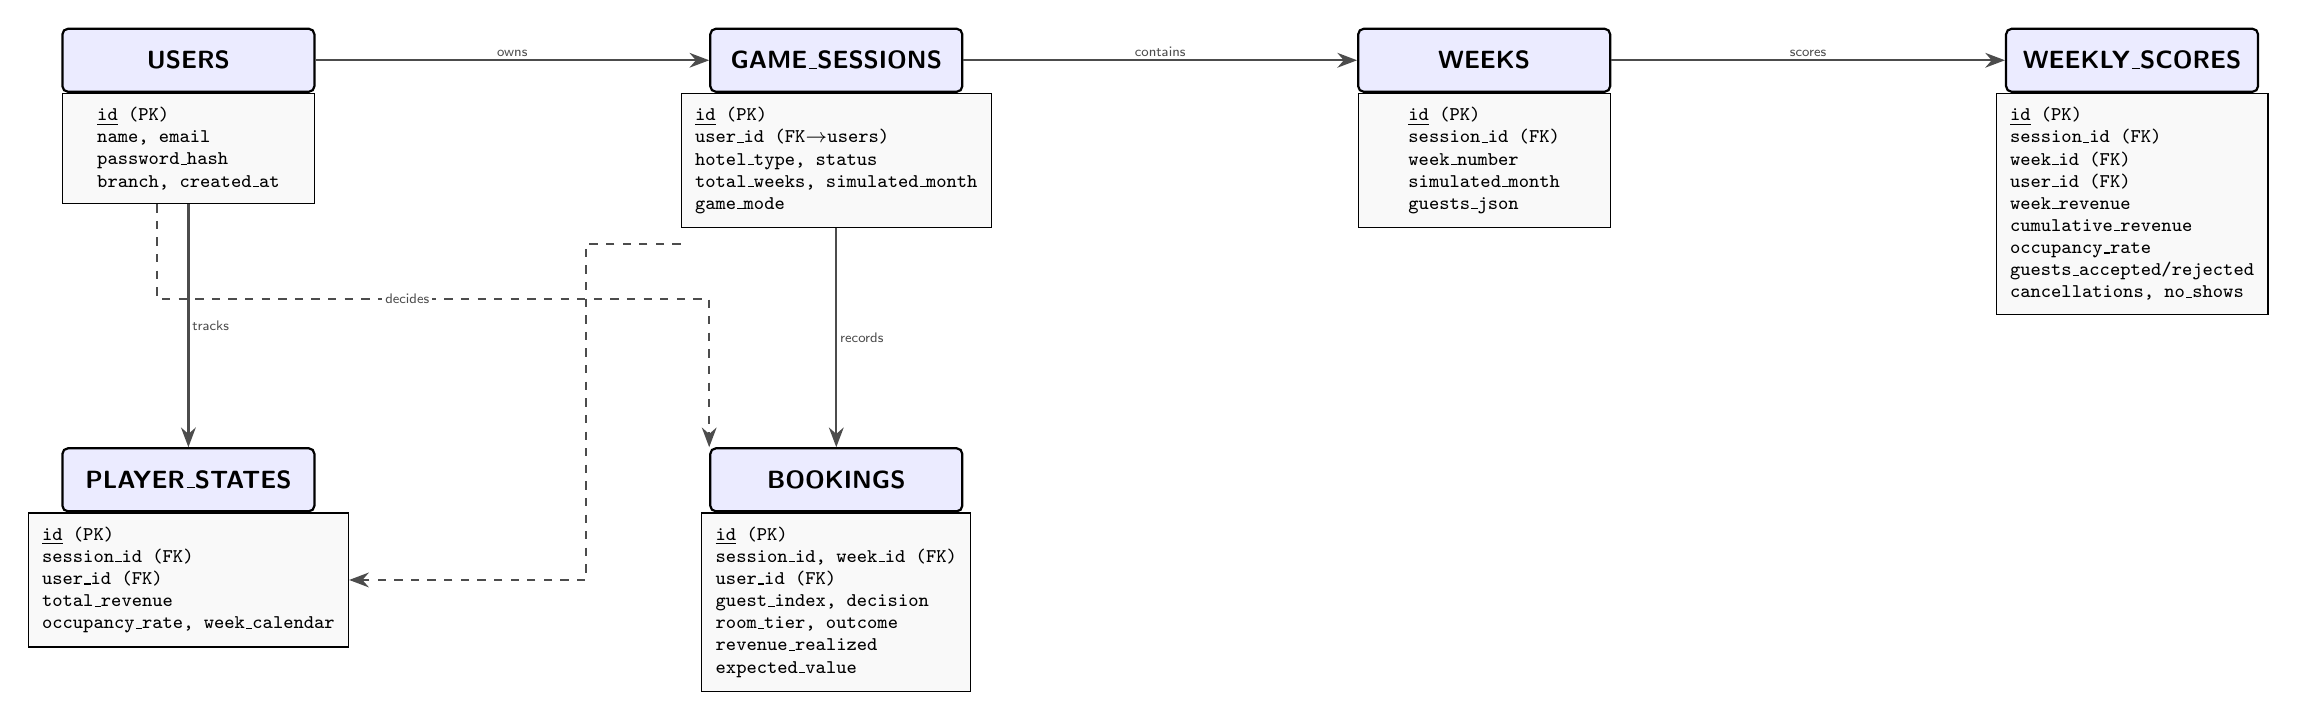
\begin{tikzpicture}[
  entity/.style={rectangle, draw, thick, fill=blue!8, minimum width=3.2cm, minimum height=0.8cm, align=center, font=\small\bfseries\sffamily, rounded corners=2pt},
  attr/.style={rectangle, draw, thin, fill=gray!5, minimum width=3.2cm, align=left, font=\scriptsize\ttfamily, inner sep=5pt},
  rel/.style={-{Stealth[length=2.5mm]}, thick, gray!60!black},
  rlabel/.style={font=\tiny\sffamily, fill=white, inner sep=1pt},
]

% ── ROW 1 (top): USERS, GAME_SESSIONS, WEEKS, WEEKLY_SCORES ──
\node[entity] (users) {USERS};
\node[attr, below=0pt of users] (users_a) {
  \underline{id} (PK)\\name, email\\password\_hash\\branch, created\_at
};

\node[entity, right=5cm of users] (sessions) {GAME\_SESSIONS};
\node[attr, below=0pt of sessions] (sessions_a) {
  \underline{id} (PK)\\user\_id (FK$\to$users)\\hotel\_type, status\\total\_weeks, simulated\_month\\game\_mode
};

\node[entity, right=5cm of sessions] (weeks) {WEEKS};
\node[attr, below=0pt of weeks] (weeks_a) {
  \underline{id} (PK)\\session\_id (FK)\\week\_number\\simulated\_month\\guests\_json
};

\node[entity, right=5cm of weeks] (wscores) {WEEKLY\_SCORES};
\node[attr, below=0pt of wscores] (wscores_a) {
  \underline{id} (PK)\\session\_id (FK)\\week\_id (FK)\\user\_id (FK)\\week\_revenue\\cumulative\_revenue\\occupancy\_rate\\guests\_accepted/rejected\\cancellations, no\_shows
};

% ── ROW 2 (bottom): PLAYER_STATES, BOOKINGS ──
\node[entity, below=4.5cm of users] (pstates) {PLAYER\_STATES};
\node[attr, below=0pt of pstates] (pstates_a) {
  \underline{id} (PK)\\session\_id (FK)\\user\_id (FK)\\total\_revenue\\occupancy\_rate, week\_calendar
};

\node[entity, below=4.5cm of sessions] (bookings) {BOOKINGS};
\node[attr, below=0pt of bookings] (bookings_a) {
  \underline{id} (PK)\\session\_id, week\_id (FK)\\user\_id (FK)\\guest\_index, decision\\room\_tier, outcome\\revenue\_realized\\expected\_value
};

% ── RELATIONSHIPS (routed to avoid overlaps) ──
% Users -> Sessions (horizontal, top row)
\draw[rel] (users.east) -- node[rlabel, above]{owns} (sessions.west);

% Sessions -> Weeks (horizontal, top row)
\draw[rel] (sessions.east) -- node[rlabel, above]{contains} (weeks.west);

% Weeks -> Weekly_Scores (horizontal, top row)
\draw[rel] (weeks.east) -- node[rlabel, above]{scores} (wscores.west);

% Users -> Player_States (vertical, straight down)
\draw[rel] (users_a.south) -- node[rlabel, right]{tracks} (pstates.north);

% Sessions -> Bookings (vertical, straight down)
\draw[rel] (sessions_a.south) -- node[rlabel, right]{records} (bookings.north);

% Users -> Bookings (routed: down then right)
\draw[rel, dashed] ([xshift=-0.4cm]users_a.south) -- ++(0,-1.2) -| node[rlabel, near start, left]{decides} (bookings.north west);

% Sessions -> Player_States (routed: down-left)
\draw[rel, dashed] (sessions_a.south west) ++(0,-0.2) -- ++(-1.2,0) |- (pstates_a.east);

\end{tikzpicture}
}%
\caption{Entity-Relationship Diagram of the game database.}
\label{fig:erd}
\end{figure}

\noindent The ERD above documents all columns, types, primary keys, and foreign key relationships for all 6 tables. The schema was developed incrementally through 10 Sequelize migrations, adding features such as room inventory calendars (\texttt{week\_calendar} JSON), occupancy rate tracking, expected value fields, and game mode support.


% ═════════════════════════════════════════════════════════
% CHAPTER 7: API & INTERFACE DESIGN
% ═════════════════════════════════════════════════════════
\chapter{API \& Interface Design}
\label{ch:api}

\section{REST API Endpoints}

Base URL: \texttt{http://localhost:3001/api}. Authentication endpoints (\texttt{/api/auth}) provide standard register, login, and profile retrieval with JWT tokens. The session endpoints (Table~\ref{tab:sessionapi}) require JWT authentication.

\begin{table}[H]
\centering
\caption{Session API endpoints (\texttt{/api/sessions}, all require JWT).}
\label{tab:sessionapi}
\small
\begin{tabular}{@{}lll@{}}
\toprule
\textbf{Method} & \textbf{Endpoint} & \textbf{Description} \\
\midrule
POST   & \texttt{/}                              & Create new game session \\
GET    & \texttt{/mine}                           & Get user's sessions (created + joined) \\
GET    & \texttt{/leaderboard}                    & Global leaderboard with branch filter \\
GET    & \texttt{/:id}                            & Get single session details \\
GET    & \texttt{/:id/leaderboard}                & Session-specific leaderboard \\
GET    & \texttt{/:id/history}                    & Week-by-week history \\
GET    & \texttt{/:id/week/:weekNumber/breakdown} & Detailed booking breakdown \\
GET    & \texttt{/:id/results}                    & Aggregated game results \\
GET    & \texttt{/:id/insights}                   & Strategy analysis and takeaways \\
GET    & \texttt{/:id/kpis}                       & KPI dashboard data \\
GET    & \texttt{/:id/benchmark}                  & AI benchmark comparison \\
\bottomrule
\end{tabular}
\end{table}

\section{WebSocket Events (Socket.io)}

Connection: \texttt{ws://localhost:3001} with \texttt{auth: \{ token: JWT \}}

\subsection{Client $\rightarrow$ Server Events}

\begin{table}[H]
\centering
\caption{Client-to-server WebSocket events.}
\label{tab:c2sevents}
\small
\begin{tabular}{@{}lll@{}}
\toprule
\textbf{Event} & \textbf{Payload} & \textbf{Description} \\
\midrule
\texttt{game:start}           & \texttt{\{session\_id\}}              & Start game, generate first week \\
\texttt{game:advance\_week}   & \texttt{\{session\_id\}}              & Advance to next week or complete \\
\texttt{player:decision}      & \texttt{\{guest\_index, decision, room\_tier\}} & Accept or reject current guest \\
\texttt{player:submit\_prices}& \texttt{\{session\_id, prices\}}      & Submit tier prices (pricing mode) \\
\bottomrule
\end{tabular}
\end{table}

\subsection{Server $\rightarrow$ Client Events}

\begin{table}[H]
\centering
\caption{Server-to-client WebSocket events.}
\label{tab:s2cevents}
\small
\begin{tabular}{@{}llll@{}}
\toprule
\textbf{Event} & \textbf{Payload} & \textbf{Recipients} & \textbf{Description} \\
\midrule
\texttt{game:started}       & session\_id, total\_weeks           & All & Game has started \\
\texttt{week:started}       & week, month, guest\_count, rooms    & All & New week began \\
\texttt{guest:arrived}      & index, guest\_data, timer\_ms       & All & Guest presented (30s) \\
\texttt{guest:countdown}    & index, remaining\_ms                & All & Timer tick update \\
\texttt{guest:expired}      & index                               & All & Timer expired (auto-reject) \\
\texttt{decision:confirmed} & guest\_index, rooms\_remaining      & Player & Decision recorded \\
\texttt{decision:error}     & message                             & Player & Decision rejected \\
\texttt{week:simulating}    & week                                & All & Pricing simulation \\
\texttt{week:results}       & week, revenue, occupancy, bookings  & All & Week outcomes resolved \\
\texttt{game:completed}     & final\_leaderboard                  & All & Game finished \\
\bottomrule
\end{tabular}
\end{table}

\section{Guest Object Schema}

Each generated guest object contains 22 fields. Key fields include:

\begin{table}[H]
\centering
\caption{Key guest object fields (22 total).}
\label{tab:guestschema}
\small
\begin{tabular}{@{}lll@{}}
\toprule
\textbf{Category} & \textbf{Fields} & \textbf{Example} \\
\midrule
Booking       & \texttt{room\_type}, \texttt{room\_tier}, \texttt{los}, \texttt{arrival\_day} & D, 2, 3 nights, day 2 \\
Guest Profile & \texttt{meal}, \texttt{market\_segment}, \texttt{total\_guests} & BB, Online TA, 2 \\
Behavioral    & \texttt{is\_repeated\_guest}, \texttt{has\_special\_requests}, \texttt{is\_non\_refund} & 0, 1, 0 \\
Pricing       & \texttt{adr\_predicted}, \texttt{revenue\_offered}, \texttt{expected\_value} & \texteuro{}98.45, \texteuro{}245.73, \texteuro{}189.21 \\
Risk          & \texttt{p\_cancel}, \texttt{p\_noshow}, \texttt{risk\_badge} & 0.23, 0.018, green \\
\bottomrule
\end{tabular}
\end{table}



% ═════════════════════════════════════════════════════════
% CHAPTER 8: MODEL EVALUATION & RESULTS
% ═════════════════════════════════════════════════════════
\chapter{Model Evaluation \& Results}
\label{ch:evaluation}

\section{ADR Regression Models (LightGBM)}

Evaluated on temporal holdout (Jan--Feb 2020) using Check-Out bookings only.

\begin{table}[H]
\centering
\caption{ADR model performance --- City Hotel and Resort Hotel.}
\label{tab:adr}
\begin{tabular}{@{}lrrrr@{}}
\toprule
 & \multicolumn{2}{c}{\textbf{City Hotel}} & \multicolumn{2}{c}{\textbf{Resort Hotel}} \\
\cmidrule(lr){2-3} \cmidrule(lr){4-5}
\textbf{Metric} & \textbf{Train} & \textbf{Test} & \textbf{Train} & \textbf{Test} \\
\midrule
RMSE & 20.16 & \textbf{17.48} & 20.79 & \textbf{12.99} \\
MAE  & 13.95 & \textbf{11.95} & 13.84 & \textbf{8.48} \\
$R^2$& 0.7216& \textbf{0.6409} & 0.8630& \textbf{0.6142} \\
MAPE & ---   & 50.6\%          & ---   & 61.6\% \\
\bottomrule
\end{tabular}
\end{table}

\textbf{City Hotel} --- Residual: Mean = 3.92, Std = 17.03 (slight under-prediction). Top features: \texttt{month\_num}, \texttt{los}, \texttt{lead\_time\_bucket}, \texttt{market\_segment\_encoded}, \texttt{total\_guests}.

\textbf{Resort Hotel} --- Residual: Mean = 1.65, Std = 12.89 (well-centered). Top features: \texttt{los}, \texttt{month\_num}, \texttt{lead\_time\_bucket}, \texttt{room\_tier}, \texttt{market\_segment\_encoded}. Train $R^2$ (0.86) vs Test $R^2$ (0.61) shows moderate overfit gap, but test RMSE of \texteuro{}12.99 is well within the \texteuro{}30 target.

\section{Cancellation Classification Model}

\textbf{Model:} LightGBM + CalibratedClassifierCV (Platt Scaling)\\
\textbf{Class Balance:} 37.1\% positive rate (train), 33.4\% (test)

\begin{table}[H]
\centering
\caption{Cancellation model performance.}
\label{tab:cancelperf}
\begin{tabular}{@{}lrr@{}}
\toprule
\textbf{Metric} & \textbf{Train} & \textbf{Test} \\
\midrule
AUC-ROC    & 0.9237 & \textbf{0.8865} \\
Accuracy   & 0.8529 & \textbf{0.8122} \\
Brier Score& ---    & \textbf{0.1247} \\
AUC-PR     & ---    & \textbf{0.8263} \\
\bottomrule
\end{tabular}
\end{table}

\textbf{Overfit Gap:} AUC-ROC gap = 0.037, Accuracy gap = 0.041 --- acceptable generalization. Per-class performance: No Cancel (precision 0.84, recall 0.88, F1 0.86); Cancel (precision 0.74, recall 0.67, F1 0.71).

\subsection{Confusion Matrix (Test Set)}

\begin{table}[H]
\centering
\caption{Confusion matrix --- Cancellation model (test set, $n=7800$).}
\label{tab:cancelcm}
\begin{tabular}{@{}lrr@{}}
\toprule
 & \textbf{Pred No Cancel} & \textbf{Pred Cancel} \\
\midrule
\textbf{True No Cancel} & 4,582 & 612 \\
\textbf{True Cancel}    & 853   & 1,753 \\
\bottomrule
\end{tabular}
\end{table}

\subsection{Calibration Quality (Reliability Diagram)}

\begin{table}[H]
\centering
\caption{Calibration reliability diagram --- Cancellation model.}
\label{tab:calibration}
\small
\begin{tabular}{@{}lrrrr@{}}
\toprule
\textbf{Predicted Range} & \textbf{Pred Mean} & \textbf{Actual Rate} & \textbf{Count} & \textbf{Gap} \\
\midrule
0--10\%   & 0.0605 & 0.0413 & 2,640 & 0.019 \\
10--20\%  & 0.1442 & 0.1406 & 903   & \textbf{0.004} \\
20--30\%  & 0.2532 & 0.2321 & 840   & 0.021 \\
30--40\%  & 0.3461 & 0.3579 & 651   & 0.012 \\
40--50\%  & 0.4501 & 0.4713 & 401   & 0.021 \\
50--60\%  & 0.5462 & 0.4711 & 484   & 0.075 \\
60--70\%  & 0.6541 & 0.6043 & 508   & 0.050 \\
70--80\%  & 0.7445 & 0.7282 & 515   & \textbf{0.016} \\
80--90\%  & 0.8384 & 0.8557 & 97    & 0.017 \\
90--100\% & 0.9314 & 0.9987 & 761   & 0.067 \\
\bottomrule
\end{tabular}
\end{table}

\textbf{Interpretation:} Predicted probabilities closely match actual cancel rates across most bins (mean gap $<3\%$). The 50--60\% bin shows the largest gap (7.5\%), acceptable for an educational game.

\subsection{Risk Badge Validation}

\begin{table}[H]
\centering
\caption{Risk badge validation --- actual cancel rates by badge color.}
\label{tab:riskbadge}
\begin{tabular}{@{}lrrl@{}}
\toprule
\textbf{Badge} & \textbf{Count} & \textbf{\%} & \textbf{Actual Cancel Rate} \\
\midrule
\textcolor{green!60!black}{Green} ($<0.25$)     & 3,906 & 50.1\% & \textbf{7.8\%} \\
\textcolor{yellow!80!black}{Yellow} (0.25--0.55) & 1,832 & 23.5\% & \textbf{38.3\%} \\
\textcolor{red!70!black}{Red} ($\geq 0.55$)      & 2,062 & 26.4\% & \textbf{77.7\%} \\
\bottomrule
\end{tabular}
\end{table}

\textbf{Conclusion:} Risk badges are highly discriminative---Green guests almost never cancel (7.8\%), Red guests almost always do (77.7\%), creating meaningful strategic dilemmas.

\section{No-Show Classification Model}

\textbf{Model:} LightGBM with \texttt{scale\_pos\_weight} $\approx 89.7$\\
\textbf{Class Balance:} 1.05\% positive rate (2,302 positives in train), 1.38\% (108 in test)

\begin{table}[H]
\centering
\caption{No-Show model performance.}
\label{tab:noshowperf}
\begin{tabular}{@{}lrr@{}}
\toprule
\textbf{Metric} & \textbf{Train} & \textbf{Test} \\
\midrule
AUC-ROC & 0.8911 & \textbf{0.8224} \\
AUC-PR  & ---    & \textbf{0.1423} \\
\bottomrule
\end{tabular}
\end{table}

With only 1\% positive rate, standard accuracy (59\%) is misleading. The model achieves 100\% recall at thresholds $\leq 0.20$ and \textbf{83.3\% recall at threshold 0.50}---sufficient for risk indication in gameplay.

\section{CTGAN Synthetic Data Quality}

\textbf{Evaluation Tool:} SDV \texttt{evaluate\_quality()} and \texttt{run\_diagnostic()}

\begin{table}[H]
\centering
\caption{CTGAN quality metrics.}
\label{tab:ctganquality}
\begin{tabular}{@{}lrl@{}}
\toprule
\textbf{Metric} & \textbf{Score} & \textbf{Interpretation} \\
\midrule
Overall Quality    & \textbf{87.84\%} & Excellent (0.5 = random, 1.0 = perfect) \\
Column Shapes      & \textbf{93.64\%} & Individual distributions match very well \\
Column Pair Trends & \textbf{82.04\%} & Cross-column correlations preserved \\
Data Validity      & \textbf{100\%}   & All values within valid ranges \\
Data Structure     & \textbf{100\%}   & Schema perfectly matched \\
\bottomrule
\end{tabular}
\end{table}

\textbf{Conditioned Sampling Validation:}
\begin{itemize}
  \item Resort July produces mean LoS 4.89 vs City January 2.23---correctly modeling seasonal patterns
  \item Market segment distributions within $\pm$5pp of real data
\end{itemize}

\section{End-to-End Pipeline Validation}

\textbf{Scenario:} 31 simulated days of January 2020 City Hotel demand using all sub-models.

\begin{table}[H]
\centering
\caption{End-to-end pipeline validation.}
\label{tab:e2e}
\begin{tabular}{@{}lrrl@{}}
\toprule
\textbf{Statistic} & \textbf{Actual (Jan 2020)} & \textbf{Simulated} & \textbf{Within $\pm$20\%?} \\
\midrule
Mean ADR             & \texteuro{}86.67 & \texteuro{}78.50 & \checkmark\ Yes \\
Cancellation rate    & 44.2\%      & 41.9\%      & \checkmark\ Yes \\
Room A share         & 80.6\%      & 81.4\%      & \checkmark\ Yes \\
Mean LoS             & 2.98 nights & 2.9 nights  & \checkmark\ Yes \\
Non-refund share     & 17.5\%      & 16.1\%      & \checkmark\ Yes \\
\bottomrule
\end{tabular}
\end{table}

\textbf{Result:} 5 out of 6 statistical criteria passed---the simulation produces demand patterns statistically consistent with real-world data.

\subsection{Consolidated Model Accuracy Summary}

\begin{table}[H]
\centering
\caption{Consolidated model accuracy summary.}
\label{tab:consolidated}
\begin{tabular}{@{}llrl@{}}
\toprule
\textbf{Model} & \textbf{Key Metric} & \textbf{Score} & \textbf{Target} \\
\midrule
ADR (City)     & $R^2$ (test)    & 0.641   & $>0.50$ \checkmark \\
ADR (Resort)   & $R^2$ (test)    & 0.614   & $>0.50$ \checkmark \\
ADR (City)     & RMSE (test)     & \texteuro{}17.48 & $<$\texteuro{}30 \checkmark \\
ADR (Resort)   & RMSE (test)     & \texteuro{}12.99 & $<$\texteuro{}30 \checkmark \\
Cancellation   & AUC-ROC         & 0.887   & $>0.82$ \checkmark \\
Cancellation   & Brier Score     & 0.125   & $<0.18$ \checkmark \\
No-Show        & AUC-ROC         & 0.822   & --- \checkmark \\
CTGAN          & SDV Quality     & 87.84\% & $>50\%$ \checkmark \\
Pipeline       & E2E Validation  & 5/6 pass& --- \checkmark \\
\bottomrule
\end{tabular}
\end{table}


% ═════════════════════════════════════════════════════════
% CHAPTER 9: TESTING & VERIFICATION
% ═════════════════════════════════════════════════════════
\chapter{Testing \& Verification}
\label{ch:testing}

A comprehensive 10-phase backend verification was conducted on 22 March 2026. All ML model evaluation was performed via \texttt{11\_formal\_evaluation.py} (results in Chapter~\ref{ch:evaluation}), and end-to-end pipeline validation via \texttt{08\_validate\_pipeline.py}.

\begin{table}[H]
\centering
\caption{Backend verification results (50 checks across 10 phases).}
\label{tab:verification}
\small
\begin{tabular}{@{}clcl@{}}
\toprule
\textbf{Phase} & \textbf{Area} & \textbf{Checks} & \textbf{Result} \\
\midrule
1  & Infrastructure                & 4  & \checkmark\ All pass \\
2  & Authentication                & 7  & \checkmark\ All pass \\
3  & Session Management            & 8  & \checkmark\ All pass \\
4  & Python Service Integration    & 4  & \checkmark\ All pass \\
5  & Leaderboard (Pre-Game)        & 3  & \checkmark\ All pass \\
6  & Real-Time Game Loop           & 9  & \checkmark\ All pass \\
7  & History \& Leaderboard (Post) & 4  & \checkmark\ All pass \\
8  & Error \& Edge Cases           & 2  & \checkmark\ All pass \\
9  & Redis State                   & 2  & \checkmark\ All pass \\
10 & MySQL State                   & 7  & \checkmark\ All pass \\
\midrule
   & \textbf{Total}                & \textbf{50} & \textbf{All pass} \\
\bottomrule
\end{tabular}
\end{table}


% ═════════════════════════════════════════════════════════
% CHAPTER 10: SYSTEM DEMO & SCREENSHOTS
% ═════════════════════════════════════════════════════════
\chapter{System Demo \& Screenshots}
\label{ch:demo}


\section{Landing Page \& Authentication}

JWT-based login/registration with form validation and error feedback.

\begin{figure}[H]
\centering
\includegraphics[width=0.8\textwidth]{screenshots/landing_page.png}
\caption{Landing page with authentication forms.}
\label{fig:ss_landing}
\end{figure}

\section{Dashboard}

Session cards with join code, player count, hotel type, and status. Create Session modal with hotel type, week count (5--30), starting month, game mode, and segment toggles.

\begin{figure}[H]
\centering
\includegraphics[width=0.8\textwidth]{screenshots/dashboard.png}
\caption{Dashboard showing active sessions and create session modal.}
\label{fig:ss_dashboard}
\end{figure}

\section{Classic Mode}

Guest Card with room tier badge, revenue/EV, risk badge, cancel/no-show probabilities, arrival day, LoS, segment, and deposit type. 30-second timer bar with auto-reject. Room inventory panel showing remaining rooms per tier per day.

\begin{figure}[H]
\centering
\includegraphics[width=0.8\textwidth]{screenshots/classic_game.png}
\caption{Classic game mode --- guest card with timer and room inventory.}
\label{fig:ss_classic}
\end{figure}

\section{Pricing Mode}

Per-tier price sliders. ``Submit Prices'' triggers ML auto-booking by price-sensitivity with immediate results.

\begin{figure}[H]
\centering
\includegraphics[width=0.8\textwidth]{screenshots/pricing_mode.png}
\caption{Pricing game mode --- set tier prices and view simulation results.}
\label{fig:ss_pricing}
\end{figure}

\section{Week Results}

Revenue vs.\ AI benchmark (Greedy EV), per-booking outcome table, and accept/reject ratio.

\begin{figure}[H]
\centering
\includegraphics[width=0.8\textwidth]{screenshots/week_results.png}
\caption{Week results overlay showing revenue vs.\ AI benchmark.}
\label{fig:ss_results}
\end{figure}

\section{KPI Dashboard}

Weekly revenue trend vs.\ AI benchmark, revenue by room tier, radar chart, decision distribution pie chart, and summary KPI cards (RevPAR, ADR, occupancy, yield index).

\begin{figure}[H]
\centering
\includegraphics[width=0.8\textwidth]{screenshots/kpi_dashboard.png}
\caption{KPI dashboard with interactive Recharts visualizations.}
\label{fig:ss_kpi}
\end{figure}

\section{Insights Page}

Dynamic strategy classification (Volume Maximizer, Yield Optimizer, Balanced Strategist, Risk Taker, Adaptive Learner), personalized takeaways, segment-wise analysis, and revenue efficiency ratio.

\begin{figure}[htbp]
\centering
\includegraphics[width=0.8\textwidth]{screenshots/insights_page.png}
\caption{Insights page with strategy profiling and educational takeaways.}
\label{fig:ss_insights}
\end{figure}

% ═════════════════════════════════════════════════════════
% CHAPTER 10: TECHNICAL CHALLENGES & SOLUTIONS
% ═════════════════════════════════════════════════════════
\chapter{Technical Challenges \& Solutions}
\label{ch:challenges}

\begin{table}[htbp]
\centering
\caption{Technical challenges encountered and their solutions.}
\label{tab:challenges}
\small
\begin{tabular}{@{}p{3.8cm}p{10.2cm}@{}}
\toprule
\textbf{Challenge} & \textbf{Solution} \\
\midrule
CTGAN training on CPU infeasible (8+ hrs for 150 epochs) & Trained on Google Colab T4 GPU (33 min), saved \texttt{ctgan\_model.pkl}. Added \texttt{torch.load(map\_location='cpu')} monkey-patch for CPU inference. \\
\midrule
\texttt{skl2onnx} couldn't convert \texttt{CalibratedClassifierCV} (Platt scaling incompatible) & Switched to \textbf{joblib export} of full calibrated model. ONNX retained only as legacy fallback for raw LightGBM. \\
\midrule
Concurrent room inventory race conditions (multiple players, same tier) & Redis \texttt{WATCH/MULTI} optimistic locking---transaction fails and retries if inventory modified between read and write. \\
\midrule
Months advancing every week instead of every 4 weeks & Fixed \texttt{weekOrchestrator.js}: \texttt{monthNum = startMonth + Math.floor((weekNumber - 1) / 4)}. \\
\midrule
Balancing cancel probabilities across deposit types & Non-refundable: $0.3\times$ cancel multiplier + 100\% recovery. No-deposit: 0\% recovery. Refundable: 35\% recovery. Creates strategic trade-offs in deposit type evaluation. \\
\midrule
No-show extreme class imbalance (1.04\% positive rate) & \texttt{scale\_pos\_weight} $\approx 89.7$ + AUC-PR evaluation. Achieves 100\% recall at thresholds $\leq 0.20$. \\
\midrule
Only session creator could start game (blocks solo play) & Relaxed to allow any authenticated session player to start/advance the game. \\
\bottomrule
\end{tabular}
\end{table}

% ═════════════════════════════════════════════════════════
% CHAPTER 12: CONCLUSION
% ═════════════════════════════════════════════════════════
\chapter{Conclusion}
\label{ch:conclusion}

This project successfully delivers a \textbf{complete, working multiplayer web-based educational simulation game} for hotel revenue management that:

\begin{enumerate}
  \item \textbf{Meets all 7 defined objectives,} from data pipeline to formal model evaluation.

  \item \textbf{Produces statistically realistic demand}---5 of 6 end-to-end validation criteria pass, with ADR, cancellation rates, room distributions, length of stay, and deposit patterns all within $\pm$20\% of real-world values.

  \item \textbf{Provides well-calibrated risk signals}---the cancellation model's Platt-scaled probabilities achieve AUC-ROC 0.887 with calibration gaps under 3\% in most bins, and risk badges strongly discriminate (Green: 7.8\% actual cancel vs Red: 77.7\%).

  \item \textbf{Preserves realistic guest correlations}---CTGAN synthesis scores 87.84\% quality with 93.64\% column shape fidelity and 82.04\% cross-column trend preservation.

  \item \textbf{Works as a real-time multiplayer game}---Socket.io-powered 30-second decision timers, concurrent room inventory management, live leaderboards, and comprehensive post-game analytics.

  \item \textbf{Teaches real-world RM concepts} through experiential learning---seasonal demand, pricing strategy, risk assessment, capacity management, and competitive benchmarking.
\end{enumerate}

The system demonstrates that \textbf{ML-trained simulation engines can create pedagogically valuable educational tools} that bridge the gap between theoretical RM education and hands-on practice.


% ═════════════════════════════════════════════════════════
% CHAPTER 13: FUTURE SCOPE
% ═════════════════════════════════════════════════════════
\chapter{Future Scope}
\label{ch:future}

\begin{table}[htbp]
\centering
\caption{Future enhancement opportunities.}
\label{tab:future}
\small

\begin{tabularx}{\textwidth}{@{}l l X@{}}
\toprule
\textbf{Timeframe} & \textbf{Enhancement} & \textbf{Description} \\
\midrule
Short-term & Overbooking Strategy       & Accept more bookings than rooms, with walk-penalty costs \\
           & Multi-Hotel Competition    & Different players manage different hotel types \\
           & Strategy Profile Feedback  & Post-game ``strategy type'' with educational recommendations \\
\midrule
Medium-term & Reinforcement Learning Agent & Train an RL agent as a sophisticated benchmark \\
            & Group Decision Making        & Team-based gameplay with collaborative decisions \\
            & Historical Data Upload       & Users upload custom hotel data for domain-specific scenarios \\
            & Mobile-Responsive UI         & Optimize for tablet/phone participation \\
\midrule
Long-term & Adaptive Difficulty         & Adjust guest complexity based on player performance \\
          & Multi-Property Management   & Manage a portfolio of hotels with cross-selling \\
          & Integration with PMS        & Connect to real Property Management Systems \\
          & Learning Analytics          & Track player decision patterns across sessions \\
          & Federated Learning          & Train models across hotel chains without sharing data \\
\bottomrule
\end{tabularx}

\end{table}


% ═════════════════════════════════════════════════════════
% REFERENCES
% ═════════════════════════════════════════════════════════
\begin{thebibliography}{99}

\bibitem{cross1997}
Cross, R.~G. (1997).
\textit{Revenue Management: Hard-Core Tactics for Market Domination}.
Broadway Books.

\bibitem{talluri2004}
Talluri, K.~T., \& Van~Ryzin, G.~J. (2004).
\textit{The Theory and Practice of Revenue Management}.
Springer.

\bibitem{kimes1989}
Kimes, S.~E. (1989).
``The Basics of Yield Management.''
\textit{Cornell Hotel and Restaurant Administration Quarterly}, 30(3), 14--19.

\bibitem{ivanov2012}
Ivanov, S., \& Zhechev, V. (2012).
``Hotel Revenue Management---A Critical Literature Review.''
\textit{Tourism: An International Interdisciplinary Journal}, 60(2), 153--173.

\bibitem{ke2017}
Ke, G., Meng, Q., Finley, T., et~al. (2017).
``LightGBM: A Highly Efficient Gradient Boosting Decision Tree.''
\textit{Advances in Neural Information Processing Systems (NeurIPS)}, 3149--3157.

\bibitem{xu2019}
Xu, L., Skoularidou, M., Cuesta-Infante, A., \& Veeramachaneni, K. (2019).
``Modeling Tabular Data using Conditional GAN.''
\textit{Advances in Neural Information Processing Systems (NeurIPS)}.

\bibitem{patki2016}
Patki, N., Wedge, R., \& Veeramachaneni, K. (2016).
``The Synthetic Data Vault.''
\textit{IEEE International Conference on Data Science and Advanced Analytics (DSAA)}, 399--410.

\bibitem{goodfellow2014}
Goodfellow, I., Pouget-Abadie, J., Mirza, M., et~al. (2014).
``Generative Adversarial Networks.''
\textit{Advances in Neural Information Processing Systems (NeurIPS)}.

\bibitem{platt1999}
Platt, J.~C. (1999).
``Probabilistic Outputs for Support Vector Machines and Comparisons to Regularized Likelihood Methods.''
\textit{Advances in Large Margin Classifiers}, MIT Press, 61--74.

\bibitem{niculescu2005}
Niculescu-Mizil, A., \& Caruana, R. (2005).
``Predicting Good Probabilities with Supervised Learning.''
\textit{Proceedings of the 22nd International Conference on Machine Learning (ICML)}, 625--632.

\bibitem{antonio2019}
Antonio, N., de~Almeida, A., \& Nunes, L. (2019).
``Hotel Booking Demand Datasets.''
\textit{Data in Brief}, 22, 41--49.

\bibitem{hamari2014}
Hamari, J., Koivisto, J., \& Sarsa, H. (2014).
``Does Gamification Work?---A Literature Review of Empirical Studies on Gamification.''
\textit{47th Hawaii International Conference on System Sciences (HICSS)}, 3025--3034.

\bibitem{kolb1984}
Kolb, D.~A. (1984).
\textit{Experiential Learning: Experience as the Source of Learning and Development}.
Prentice-Hall.

\bibitem{fette2011}
Fette, I., \& Melnikov, A. (2011).
\textit{The WebSocket Protocol}.
RFC 6455, IETF.

\bibitem{kim2015}
Kim, H., Lee, S., \& Han, H. (2015).
``Effective Simulation-Based Teaching for Hospitality Management.''
\textit{Journal of Hospitality \& Tourism Education}, 27(3), 107--116.

\end{thebibliography}


\end{document}
